\TODO{add my ideas for solution}
% comparison table of various solutions
% Analyze and comment solutions
% Add out idea for solution

% summary of section:
In this section we will analyze popular solutions available in the market,
highlighting each solution strenghts and weaknesses.
Later on a table is presented summarizing each solution and relevant features compared, and its
data discused.
The section ends with the author's ideas for an alternative solution.

\subsection{AutoCAD}
AutoCAD\cite{SITE-AUTOCAD} is the \emph{de facto} standard software for architecture designs.
It has a steep learning curve (Fig.\ref{FIG-AUTOCAD}) but is nevertheless
learned all over the world.

One of its formats, DXF, is widely supported in 3D modelers and engines.
AutoCAD features a powerful language, AutoLisp, which allows advanced users to create scripts for
automating any aspect available in the interface.

This program favors 2D drawing and modeling over real 3D concepts,
but a skillful operator can create every shape necessary to an architectural scenario.
Internally AutoCAD doesn't support any interactive preview of the created designs.

It renders using the Mental Ray\nocite{SITE-MENTAL} engine.
Animations can be made using camera paths.

\begin{figure}[!ht]
    \centering
    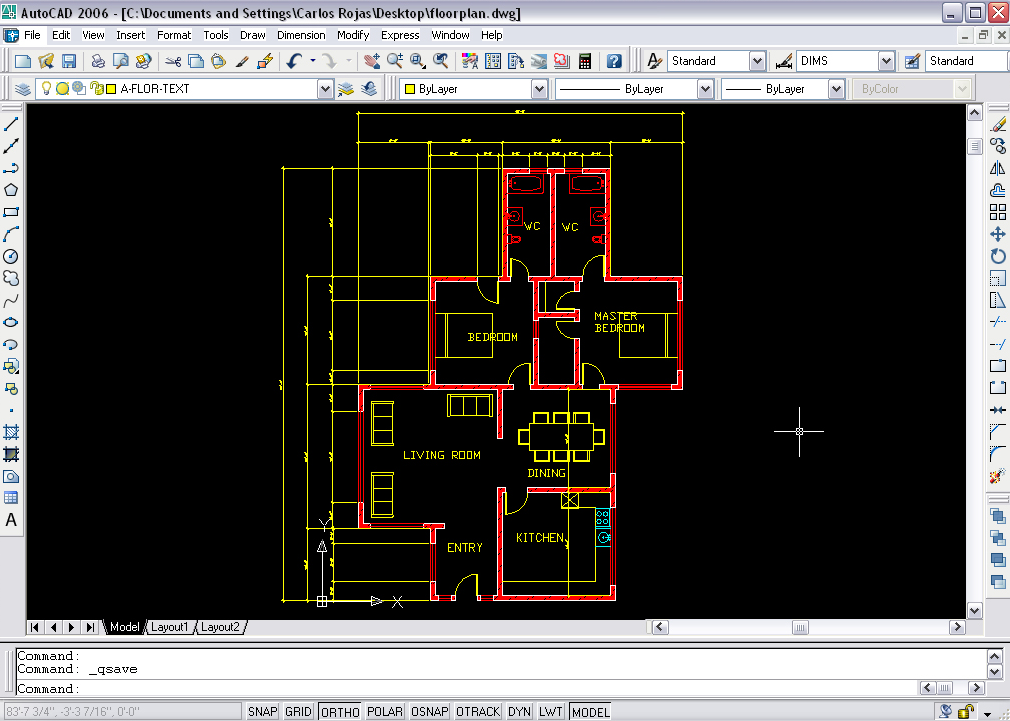
\includegraphics[width=9cm]{gfx/autocad-1.png}
    \caption{AutoCAD: A typical layout of a floor plan.}
    \label{FIG-AUTOCAD}
\end{figure}

\subsection{ArchiCAD}
GraphiCad's ArchiCAD\cite{SITE-ARCHICAD} aims at conquering new architecture students who haven't been exposed to AutoCAD.

It offers pre-made views and document templates for every architectural driven need.
It is by definition a 3D CAD program and it is praised by architects for its easy 3D
manipulation capabilities (Fig.\ref{FIG-ARCHICAD}).

The program features templates for common architectural elements.
ArchiCAD has navigation capabilities too, allowing first person perspective navigation of the model.
Its workflow is thought out to make it easy for an architect to do the most common tasks,
making it a friendlier alternative when compared to AutoCAD.
It lacks the expressive power to do about 10\% uncommon tasks though.

There's a Software Development Kit for ArchiCAD plugin creation.

\begin{figure}[!ht]
    \centering
    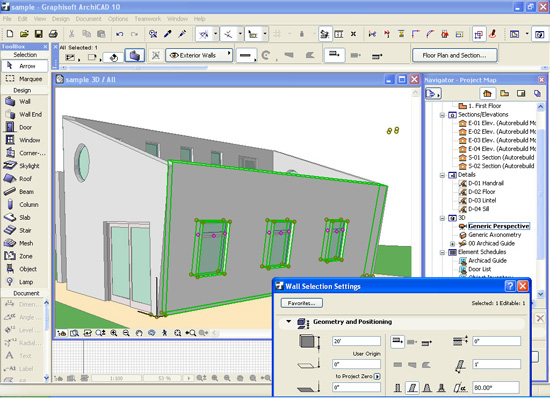
\includegraphics[width=9cm]{gfx/archicad-1.png}
    \caption{ArchiCAD: Notice basic selection and template properties editing in the 3D view.}
    \label{FIG-ARCHICAD}
\end{figure}

\subsection{Revit Building}
Revit Building\cite{SITE-REVIT} is another Autodesk product.
Unlike AutoCAD, which spans its use to other areas such as mechanical engineering,
Revit Building was explicitly thought out for architectural design.

It works completely in 3D and has native templates for doors, windows, roofs, etc.
Features the concept of mass, lacking in most packages.
Common constraints are detected. Thick walls can be drawn as lines and solids can
be cut as floors (compare the top-left and bottom right views in Fig.\ref{FIG-REVIT}).

Revit Building features powerful templates for complex tasks such as roof design.
It has a simple raytacer and radiosity engine. Cameras can be placed but only for view
rendering, not animation.

Being a system for the professional segment, it has a lower learning curve and provides
tools that allow successful modeling of complex buildings, even for enthusiasts,
something much harder to do in AutoCAD.

\begin{figure}[!ht]
    \centering
    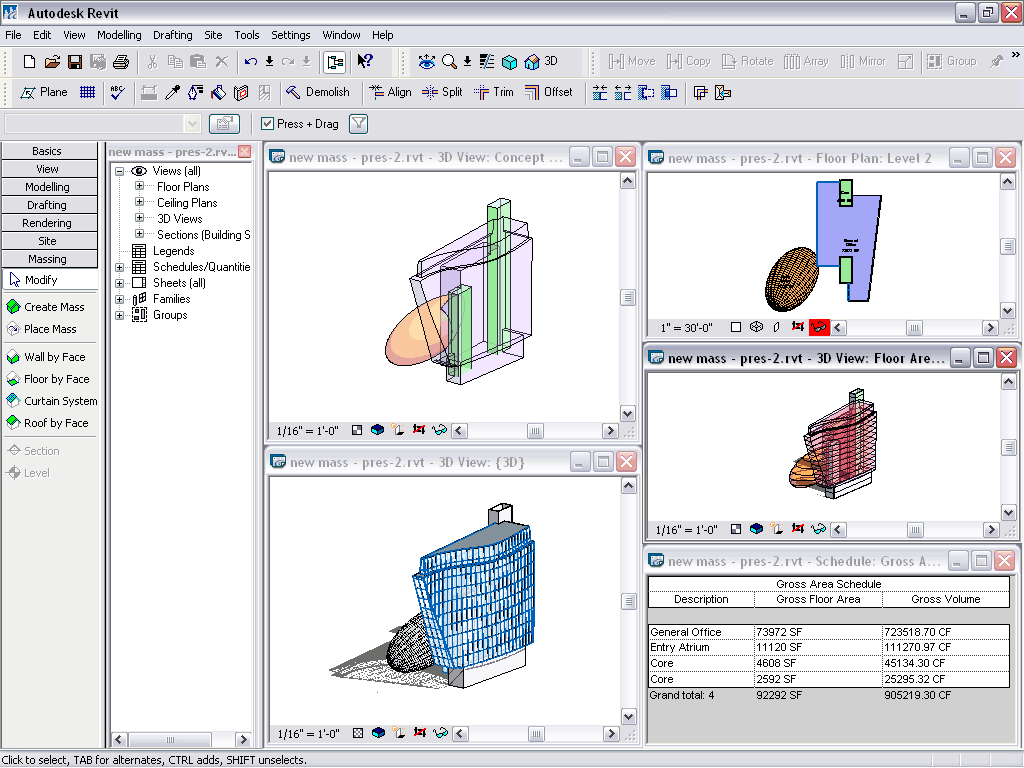
\includegraphics[width=9cm]{gfx/revit-1.png}
    \caption{Revit Building: Solid shapes can be combined with boolean operations and converted into buildings.}
    \label{FIG-REVIT}
\end{figure}

\subsection{SketchUp}
Google SketchUp \cite{SITE-SKETCHUP} is a friendly program for the novice 3D modeler.
It features a simple interface and most of its tools are basic,
still able to achieve acceptable results.
Its learning curve is great -- everyone can sketch a room in a nick of time.

Its engine is based on drawing lines on top of lines,
already created surfaces or a construction plane.
It detects the most common geometry restrictions (such as midpoint and perpendicularity).

Features an online repository of models, allowing importing of objects such as
furniture, trees, props or well known buildings by just browsing and selection.

Performs strange results when handling awkward angles or when several lines
are the vicinity of the mouse.
Curve manipulation and generation of surfaces is nonexistent.
Allows plugin design in the Ruby language.

Another bonus from being part of the Google software library, SketchUp features import/export capabilities to Google Earth\cite{SITE-EARTH}.
This allows capturing a patch of land to SketchUp, design a building there and export the patch
back with its new contents to Google Earth.

A great feature SketchUp is realtime shadows (Fig.\ref{FIG-SKETCHUP}) -- since there's only one viewport, shadows are crucial to give the user a sense of depth to a scene.

In renders cartoonish styled views and allows interpolation of cameras to render simple animations.

The professional version of the program allows exporting to common 3D architectural formats.


\begin{figure}[!ht]
    \centering
    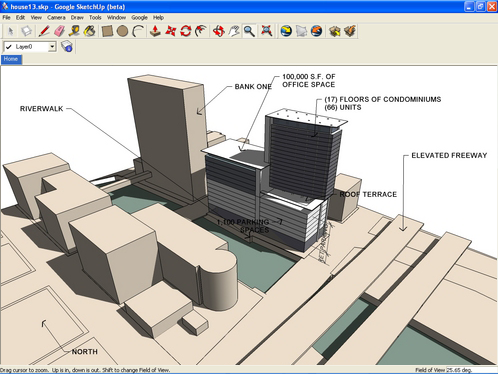
\includegraphics[width=9cm]{gfx/sketchup-1.png}
    \caption{SketchUp: Basic shape extrusions. Notice the shadows in the viewport.}
    \label{FIG-SKETCHUP}
\end{figure}

\newpage

\subsection{Comparison Table of Available Solutions}
\begin{table}[!ht]
  \centering
  \caption{Different solutions in the market compared.}
	\begin{tabular}{|c|c|c|c|c|}
		\hline
		\backslashbox{Features}{Solutions}		& AutoCAD		& ArchiCAD	& Revit Building	& SketchUp	\\
		\hline
		Design in 2D						&		\GdA		&		\GdB		&				\GdB			&		\GdC		\\
		\hline
		Design in 3D						&		\GdD		&		\GdC		&				\GdB			&		\GdB		\\
		\hline
		Architectural Templates	&		\GdD		&		\GdB		&				\GdA			&		\GdC		\\
		\hline
		Supported Formats				&		\GdC		&		\GdC		&				\GdB			&		\GdD / \GdB \footnotemark\\
		\hline
		Interactive Modes				&		\GdE		&		\GdB		&				\GdC 			&		\GdE		\\
		\hline
		Rendering Capabilities	&		\GdB		&		\GdB		&				\GdC			&		\GdD		\\
		\hline
		Extensibility						&		\GdA		&		\GdC		&				\GdE			&		\GdC		\\
		\hline
	\end{tabular}
	\label{TB-COMP-SOL}
\end{table}
\footnotetext{SketchUp exporting capabilities depend on using free or commercial version}

\begin{table}[!ht]
  \centering
  \caption{Legend of Table \ref{TB-COMP-SOL}}
	\begin{tabular}{|p{2cm}|p{2cm}|p{2cm}|p{2cm}|p{2cm}|}
		\hline
		very bad	& bad			& average	& good		& very good	\\
		\hline
			\GdE		&	\GdD		&	\GdC		&	\GdB		&	\GdA			\\
		\hline
	\end{tabular}
  \label{TB-COMP-SOL-LEGEND}
\end{table}

\subsection{Discussing the Table}
AutoCAD makes use of a well established workflow, which takes time to master.
There's a way of doing everything architecturally speaking, though most times a difficult one.
Since its a package general enough for supporting other uses, AutoCAD doesn't come with architectural
templates, a very helpful feature available in both ArchiCAD and Revit Building.

Revit Building is Autodesk's vision of an easy to master, yet powerful system for architectural design.
Revit Building and ArchiCAD are the most similar systems.
Revit Building has better modeling features while ArchiCAD has many document templates
ready for extracting bureaucratic papers out of the architect's workflow.

SketchUp is undoubtfully the most amateur of the analyzed systems.
It offers limited geometrical operations and doesn't have a real template library.
It tries to overcome that limitation by offering a large online repository of models.
SketchUp's best qualities are its learning curve -- any user can feel confident in
modeling a simple floor in a couple of minutes -- and the Google Earth connection.

It would be of great use if other programs were granted permission to get geographical
data (both height maps and texture maps) of an area on Earth.
This offers an important head start for an architect in designing a building that
smoothly blends in its surroundings.
